\chapter{Related work}
Previous works mainly focus on finding more discriminative descriptors and better metric learning. It is known that color and texture are the most important information in Re-ID. Researchers found that features based on a single attribute (like color or texture) are not robust to various datasets. Instead, combinations of different features are exploited to improve the performance. Most descriptors capture the local or global statistic color and texture information to characterize individuals. A brief introduction of those descriptors and metrics is given in this chapter.

\section{Appearance descriptors}
In most descriptors, local features \cite{Appearancedesc} are used to characterize the color, texture and other properties. The input image will be divided into a few subregions, features of those subregions are extracted respectively and concatenated directly or characterized by their statistic properties. According to how those subregions are divided, there can be three kinds of models, fixed part-based models, adaptive models and learned part models \cite{Appearancedesc}. 

In fixed part models, the size of body parts is predefined. One example is in \cite{ImportantFeatures, PRDC, REIDSVM}, where a silhouette is divided into a fixed number of horizontal stripes, which mainly include the head, torso and legs. In \cite{AppBasedREID}, the input images are divided into three horizontal stripes, and the width of each stripe is respectively 16\%, 29\% and 55\%.  The fixed models predefine parameters such as numbers of stripes and the stripe height. 

In the adaptive part models, the size of each body parts may vary to fit predefined body part models. Take \cite{SDALF} for an instance; the silhouette of each person is divided into three parts horizontally, which include the head, torso and legs respectively. But the height of each stripe is different for various silhouettes, and it is computed according to symmetry and asymmetry with two operators $C(i, \delta)$ and $S(i,\delta)$, where 
\begin{equation}
\begin{aligned}
C(i,\sigma) & = \sum_{B_{[i-\delta, i+\delta]}}{d^2(p_i-{\hat{p}_i)}}, \\
S(i,\sigma) &= \sum{\frac{1}{W\delta}|A(B_{[i,i-\delta]}) - A(B_{[i,i+\delta]})|}.
\end{aligned}
\end{equation}
Here the $C(i, \delta)$ is called the \emph{chromatic bilateral operator}, and it computes the Euclidean distance of two HSV blobs located symmetrically with respect to horizontal axis $y = i$, where $B_{[i-\delta, i+\delta]}$ is the blob with a height $2\delta$. $S(i,\delta)$ is called the \emph{spatial covering operator} and it computes the difference of two foreground areas. Then the axis between the torso and legs is computed as follow:
\begin{equation}
\begin{aligned}
i_{TL} = \mathop{\arg\min}_i(1-C(i,\delta)+S(i,\delta)),
\end{aligned}
\end{equation}
and the axis  between the head and torso is computed with the following equation:
\begin{equation}
\begin{aligned}
i_{HT} = \mathop{\arg\min}_i(-S(i,\delta)).
\end{aligned}
\end{equation}
The axis dividing the left and right torso is
\begin{equation}
\begin{aligned}
j_{LR} = \mathop{\arg\min}_j(C(j,\delta)+S(j,\delta)).
\end{aligned}
\end{equation}
This method has good performance. But one shortcoming of this model is that an imperfect background segmentation causes noise and introduces errors regarding the position of axes. \\
%-------------------------------------------------------------------------------------------------------------------------------------------------------------------------------------------------------------------------------------------------------------------
\indent Another part-based adaptive spatial-temporal model used in \cite{PartbasedSTReid} characterizes a person's appearance using color and facial features. Few works exploit human face features. In this work, human face detection based on low resolution cues selects useful face images to build face models. Color features capture representative color as well as the color distribution to build a color model. This model handles multi-shot re-identification, and it also characterizes the color distribution variation of many consecutive frames.  Besides, the facial features of this model is conditional. That is, in the absence of good face images, this model is only based on color features.

Some methods based on learned part models have been proposed. Part model detectors (statistic classifiers) are trained with manually labelled human body parts images, exploiting features related to edges contained in the images. A pictorial structure (PS) is proposed in \cite{PictorialModel}. The PS model of a non-rigid body is a collection of part models with deformable configurations and connections with certain parts. The appearance of each part is separately modelled, and deformable configurations are implemented with spring-like connections. This model can quantitatively describe visual appearance and model the non-rigid body. In \cite{PSmodelRevisit}, the pictorial structure body model is made up of N parts and N corresponding part detectors. 

Another example of the learned part model is in \cite{MultiPersonREID, PartbasedSTReid}. The overall human body model consists of several part models; each model is made up of a spatial model and a part filter. For each part, the spatial model defines allowed arrangements of this part with respect to the bounding box. To train each model, the latent support vector machine (LSVM) is used, and four body parts are detected, namely the head, left and right torso and upper legs. Compared with other models, this model exploits a sequence of frames of an individual and thus captures appearance characteristics as well as the appearance variation over time.

Features can be implemented with different methods. According to the way to extract features for a model (a whole model or a part-based model), features can be divided into two categories \cite{Appearancedesc}: global and local features. Global features refer to features extracted from a whole image or region, and the size of the descriptor is usually fixed. In order to extract local feature of a specified image or region, we first divide the whole image into many equal blocks and compute the feature of each block.  Both descriptors may deal with color, texture and shape. The color information is exploited most by extracting the color histogram within different color spaces. Descriptors based on texture, such as the scale-invariant feature transform (SIFT), speeded up robust features (SURF) and LBP, are also widely combined to improve performance.

Global color histogram is a frequently used global feature. For an three-channel image, like an RGB image, each channel is quantized into $B$ bins separately. The final histogram could be a multi-dimensional or one-dimensional histogram. For instance, if $B = 8$, for a multi-dimensional histogram, there will be  $8\times 8\times 8 = 512$ bins. But if we concatenate the three-dimensional bins together, the dimension can be reduced to $8 + 8 + 8 = 24$ bins while the performance of this reduced descriptor doesn't decrease. This method can be applied on other color spaces like HSV and Lab, etc.

Local color histogram usually splits the specified model or region into many equal-sized blocks and computes the global feature of each block. The feature can be based on color, texture and interest points. SIFT \cite{SIFT} is a kind of local feature based on the interest points. The salient interest points (identifiable over rotating and scaling) are selected by the interest operator. This algorithm detects key points by computing the difference of Gaussian ($DoG$) images of different scales $\sigma$ with the equation
\begin{equation}
D(x,y,\sigma) = (G(x,y,k_1\sigma) - G(x,y,k_2\sigma))\ast I(x,y).
\end{equation}
Here $G(x,y,k_1\sigma)$ is the Gaussian function with deviation $k_1\sigma$, $I(x,y)$ is the image. The $DoG$ images are compared to find their extrema as key points. With key points localization and other processing, descriptors describing key points are created as SIFT descriptors.

The maximally stable color region (MSCR) is used in \cite{SDALF}. The MSCR derives from the maximally stable extreme region (MSER) and detects the region with a stable color cluster. It uses an agglomerative clustering algorithm to compute color clusters, and by looking at the successive time steps of the algorithm, the extension of color is implemented. The detected color region is described with a nine-dimensional vector containing the area, averaging color, centroid and second moment matrix. With this vector, the color region detected makes it easy to do scale and affine transforms.

Recurrent highly structured patches (RHSP) is also used in \cite{SDALF}. This feature captures patches with highly recurrent color and texture characteristics from extracted silhouette pixels. This feature is extracted from the following steps. First, random and probably overlapping small image patches are extracted from silhouette pixels. Then, to capture those patches with informative texture, the entropy of each patch (the sum of the three channels' entropy) is computed, and we discard those patches with entropy smaller than a specified threshold. In the next step, some transforms are performed on the remaining patches to select those remaining invariant to the transforms. Subsequently, the recurrence of each patch is evaluated with the local normalized cross correlation (LNCC) function. This evaluation is only performed on a small region containing the patch instead of the whole image. Then the patches with high recurrence are clustered to avoid patches with similar content. Finally, the Gaussian cluster is applied to maintain the patch nearest to the centroid of each cluster for each cluster.

In \cite{SARC3D}, a new 3D model model called SARC3D  is used to characterize the individual. Compared with those 2D models, this model combines the texture and color information with their location information together to get a 3D model. This model starts with an approximate body model with a single shape parameter. By precise 3D mapping, this parameter can be learned and trained with even quite few images (even one image is feasible). This model's construction is driven by the frontal, top and side views extracted from various videos, and for each view, the silhouette of a person is extracted to construct the 3D graphical model. The final body model is sampled to get a set of vertices from the previously learned graphic body model. Compared with other models, this model has a robust performance when dealing with partial occlusion, people posture variation and viewpoint variations since the model is based on silhouettes from three viewpoints.
%--------------------------------------------------------------------------------------------------------------------------------------------------------------------------------------------------------------------------------------------------------------------------------

Descriptors combining color and texture are most often used in re-identification. In \cite{AHPE}, a signature called asymmetry-based histogram plus epitome (AHPE) was proposed. This work starts with a selection of images to reduce image redundancy, which is caused by correlated consecutive sequences. This descriptor combines global and local statistical descriptors of human appearance, focusing on overall chromatic content via histogram and on the recurrent local patches via epitome analysis. Similar to the SDALF descriptor \cite{SDALF}, the HPE descriptor consists of three components, the chromatic color histogram, the generic epitome and local epitome. The chromatic color histogram is extracted in the HSV color space, which turns to be robust to illumination changes. Here, color histogram is encoded into a 36-dimensional feature space $[H=16,  S=16,  V=4]$. The authors define epitome to be a collage of overlapped patches. This collage is generated by the collapsing of an image or a sequence of images, and this collage indicates the essence of the texture, shape and chromatic properties of the image or sequential images.

\section{Metric learning}
The second step of Re-ID is to design the metric learning to match descriptors, i.e., the way to compare how similar two descriptors are. Many different metric learning methods have been proposed \cite{KISSME, LFDA, PCCA, TDL, PRDC, LMNN, KLFDA, KCCA, KernelVersionMetrics, NFST, ITML} to get smaller intraclass distance and larger interclass distance. Generally, for two $d\times 1$-dimensional input vectors $\bm{x}_1$, $\bm{x}_2$, any symmetric positive semi-definite matrix $M$ defines a pseudo-metric with the form of $D = (\bm{x}_1 -\bm{x}_2)^T\bm{M}(\bm{x}_1 - \bm{x}_2)$. Many widely used distance metrics exploit this rule. Previous methods includes the Euclidean distance, Bhattacharyya distance and Mahalanobis distance methods. The Euclidean distance, which is the most common used distance, is a special case of Mahalanobis distance when the $\bm{M}$ is an identity matrix. One example of metric learning is the probabilistic relative distance comparison model proposed in \cite{PRDC}. This model exploits all the possible positive person pairs and negative pairs so that for each person, the between-class distance is larger than the within-class distance. Compared with the other distance learning models proposed, this model solves the matrix $\bm{M}$ by an iterative optimization algorithm. Suppose $\bm{z}$ is an image descriptor of a person; the task is to identify another image descriptor $\bm{z}'$ of the same person from $\bm{z}''$ of a different person by using a distance model $f(\cdot)$, so that $f(\bm{z}, \bm{z}')< f(\bm{z}, \bm{z}'')$. The authors convert the distance learning problem to a probability comparison problem by measuring the probability of the distance between a relevant pair of images being smaller than that of a related irrelevant pair as
\begin{equation}
P(f(\bm{z},\bm{z}')<f(\bm{z},\bm{z}'')) = (1+\exp^{(f(\bm{z}-\bm{z}')-f(\bm{z}-\bm{z}''))})^{-1}.
\end{equation}
Here the author assumes that probability of $f(\bm{z},\bm{z}')$ and $f(\bm{z},\bm{z}'')$ is independent, therefore, using the maximal likelihood principal, the optimal function can be learned as
\begin{equation}
\begin{aligned}
f &= \mathop{\arg\min}_f r(f,O), \\
r(f,O) &= -\log(\prod_{O_i}P(f(\bm{x}_i^p) < f(\bm{x}_i^n))).
\end{aligned}
\end{equation}
$O=\{O_i=(\bm{x}_i^p, \bm{x}_i^n)\}$ , $\bm{x}_i^p$, $\bm{x}_i^n$ are intraclass and interclass vector differences respectively, and $\bm{x}_i^p$, $\bm{x}_i^n$ are defined as
\begin{equation}
\begin{aligned}
\bm{x}_i^p &= |\bm{z} - \bm{z}'|, \\
\bm{x}_i^n &= |\bm{z} - \bm{z}''|.
\end{aligned}
\end{equation}
The distance function $f(\cdot)$ here is parameterized as the Mahalanobis distance function
$f=\bm{x}^T\bm{M}\bm{x},\bm{M\ge}0$. Here $\bm{M}$ is a semi-positive definite (SPD) matrix. In this way, the distance function learning problem is transformed to a matrix optimization problem. The author used an iteration algorithm to compute matrix $\bm{M}$. One shortcoming for this algorithm is that it is computationally expensive because for each person it compares distances between all the possible negative pairs and corresponding positive pairs. 

Single-shot image-based person representation suffers from the small sample size problem. This is why multi-shot Re-ID has been proposed. Since there are a sequence of images for each individual, there are many more cues to exploit.
In \cite{TDL}, the author simplified computing of the Mahananobis matrix by applying the new limitations on datasets. The author found that when using video-based person representation, the difference of interclass may be more obscure than that of still-image-based representation. Therefore, the author proposed the top-push distance learning model. For all the person pairs, the maximal intraclass distance should be one unit smaller than the minimal distance of interclass distance. Another constraint introduced the sum of all intraclass distance should be as small as possible, so the final target function is summarized as:
\begin{equation}
\begin{aligned}
f(D) = (1-\alpha)\sum_{\bm{x}_i,\bm{x}_j,y_i=y_j} D(\bm{x}_i,\bm{x}_j) + \\
\alpha \sum_{\bm{x}_i,\bm{x}_j,y_i=y_j}\max\{{D(\bm{x}_i,\bm{x}_j)-\min_{y_i\ne y_k}{D(\bm{x}_i,\bm{x}_k)}+\rho,0}\}.
\end{aligned}
\end{equation}
Here, $\bm{x}_i, \bm{x}_j and \bm{x}_k$ are feature descriptors, and $y_i, y_j and y_k$ are class labels.

Some previous works exploit the Fisher discriminant analysis and convert the problem to a matrix eigenvalue decomposition problem. In \cite{LFDA}, the local fisher discriminant analysis (LFDA) is used, and in \cite{KernelVersionMetrics}, the kernel version of several linear metrics are proposed, and it proves that kernelization improves Re-ID performance. In \cite{LOMO}, the log ratio of Bayesian-based estimation is proposed to have advanced performance. In \cite{NFST}, the authors propose to make sample points of the same class collapse to the same point in the null space while different points are project to different points. In \cite{SCNCD}, the semantic representation of color names is exploited. In this thesis, an SPD matrix $\bm{M}$ is learned to meet certain intraclass and interclass distance limitations. 

\section{Other methods for Re-ID}
Besides the descriptors and metrics mentioned above, there are some other methods for Re-ID. Convolutional neural networks (CNN) have been exploited in Re-ID. One advantage of the neural network Re-ID is that the preprocessing of images can be skipped. We can also say the preprocessing is included in convolutional layers. The input of this structure can be straightforward grey images or color images.  Traditional neural networks have too many weights to train. Convolutional neural networks can avoid this problem while retaining high performance. Compared with classical neural network architecture, the convolutional neural network exploits receptive field, weights sharing and pooling to reduce weights number and thus decreases computational cost. When dealing with multi-shot and video-based re-identification, neural networks are proven to have better performance. In \cite{RecurrentCNN}, the author proposes a recurrent neural network layer and temporal pooling to combine all time-steps data to generate a feature vector of the video sequence. In \cite{MultiCNN}, the author proposes a multi-channel layer based neural network to jointly learn both local body parts and whole body information from input person images.  In \cite{DeepfeatureCNN}, a convolutional neural network learning deep feature representations from multiple domains is proposed, and this work also proposes a domain-guided dropout algorithm to dropout CNN weights when learning from different datasets. \\
\indent There are many other works based on convolutional neural networks. However, person re-identification may be one of the areas where CNN performance may be poorer than regular machine learning methods for the small sample size problem (SSS). In most datasets, the sample size of each pedestrian is quite small. Especially in single-shot Re-ID only one frame is provided in each view for each person. This is why Re-ID more often relies on classical machine learning.

%
%By learning from multiple datasets this method gives a solution to the problem that most CNNs are not trained enough caused by datasets with small number of images.

\section{Some state-of-the-art works}
Recently, many works have been proposed that improved Re-ID performance by a wide margin. In this section, those advanced descriptors and metrics are introduced. 

\textbf{Cross view quadratic discriminant analysis} (XQDA) is proposed in \cite{LOMO}. Let's define the sample difference $\Delta = \bm{x}_i - \bm{x}_j$, where $\bm{x}_i $ and $\bm{x}_j$ are two feature vectors. $\Delta$ is called intrapersonal difference when their labels satisfy $y_i = y_j$ and extrapersonal difference when $y_i \ne y_j$. The intrapersonal and interpersonal variation can be defined as $\Omega_I$ and $\Omega_E$. The authors convert the Re-ID problem to distinguishing $\Omega_I$ from $\Omega_E$. In \cite{Bayeface}, each one of intrapersonal and interpersonal class is modelled with a multivariate Gaussian distribution, and in \cite{Bayeface}, it has been proven that both $\Omega_I$ and $\Omega_E$ have zero mean. Under the zero-mean distribution, the probability of observing $\Delta$ in $\Omega_I$ and the probability of observing $\Delta$ in $\Omega_E$ can be denoted as
\begin{equation}
\begin{aligned}
P(\Delta|\Omega_I) &= \frac{1}{(2\pi)^{d/2}|\Sigma_I|^{1/2}}\exp^{\frac{-1}{2}\Delta^T\Sigma_I^{-1}\Delta},\\
P(\Delta|\Omega_E) &= \frac{1}{(2\pi)^{d/2}|\Sigma_E|^{1/2}}\exp^{\frac{-1}{2}\Delta^T\Sigma_E^{-1}\Delta},
\end{aligned}
\end{equation}
where $\Sigma_I$ and $\Sigma_E$ are the covariance matrix of $\Omega_I$ and $\Omega_E$. Then the probability ratio between the interpersonal pairs and intrapersonal pairs can be denoted as
\begin{equation}
\begin{aligned}
r(\Delta) = \frac{P(\Delta|\Omega_E)}{P(\Delta|\Omega_I)}
	   &=\frac{\frac{1}{(2\pi)^{d/2}|\Sigma_E|^{1/2}}\exp^{\frac{-1}{2}\Delta^T\Sigma_E^{-1}\Delta}}{\frac{1}{(2\pi)^{d/2}|\Sigma_I|^{1/2}}\exp^{\frac{-1}{2}\Delta^T\Sigma_I^{-1}\Delta}},\\
r(\Delta)& =  C\exp^{\frac{-1}{2}\Delta^T(\Sigma_E^{-1} - \Sigma_I^{-1})\Delta}.
\end{aligned}
\end{equation}
Here C is a constant term, and by taking the log and deserting the constant term, we have 
\begin{equation}
\begin{aligned}
r(\Delta) = \Delta^T(\Sigma_I^{-1} - \Sigma_E^{-1})\Delta 
	   & = (\bm{x}_i - \bm{x}_j)^T(\Sigma_I^{-1} - \Sigma_E^{-1})(\bm{x}_i - \bm{x}_j).
\end{aligned}
\end{equation}
In \cite{LOMO}, a subspace $W$ is learned so that 
\begin{equation}
r(\Delta) = (\bm{x}_i - \bm{x}_j)^TW({\Sigma_I}'^{-1} - {\Sigma_E}'^{-1})W^T(\bm{x}_i - \bm{x}_j),
\end{equation}
and ${\Sigma_I}' = W^T\Sigma_IW, {\Sigma_E}' = W^T\Sigma_EW$. Therefore, a subspace $M(W) = W({\Sigma_I}'^{-1} - {\Sigma_E}'^{-1})W^T$ is learned in this work.\\
\indent \textbf{Null Foley-Sammon transform (NFST)} In \cite{NFST}, a null space is proposed so that with this space the intraclass points collapse to a same point in the null space while interclass points are projected to different points. Given the within-class scatter $\bm{S}^w$ and between-class scatter $\bm{S}^b$, an optimal projection matrix $\bm{W}$ is computed so that 
\begin{equation}
\begin{aligned}
\bm{w}_i^T\bm{S}^w\bm{w}_i = 0,\\
\bm{w}_i^T\bm{S}^b\bm{w}_i > 0.
\end{aligned}
\end{equation}
Here $\bm{w}_i$ is the $i_{th}$ column in $\bm{W}$.

It can be noted that like many other metric learnings, XQDA and NFST evolve to matrix decomposition and eigenvalue selection problems. In this paper, XQDA and NFST are used to compare with the proposed metric. In \cite{GOG}, it has been shown that GOG + XQDA outperforms many other combinations, including Metric ensemble \cite{MetricEnsembles}, SCNCD \cite{SCNCD}, Semantic method \cite{SemanticMethod}, etc. In \cite{ NFST}, it has been shown LOMO + NFST outperforms metrics including LMNN \cite{LMNN}, KCCA \cite{KCCA}, ITML \cite{ITML}, KLFDA \cite{KLFDA}, MFA \cite{KernelVersionMetrics}, KISSME \cite{KISSME}, Similarity learning \cite{SimilarityLearning}, SCNCD \cite{SCNCD}, Mid-level filters \cite{MidlevelFilters} and Improved deep learning \cite{ImprovedCNN}. Based on the result that XQDA and NFST outperform other metrics, XQDA and NFST are used in this thesis to compare with our proposed metric learning. 

\section{Performance measuring}
There are a few measures of Re-ID, such as cumulative matching curve (CMC), receiver operating characteristic curve (ROC) and synthetic recognition rate (SRR). Specifically, the CMC is used as a 1:m re-identification system and ROC is used for a 1:1 re-identification system. The
SRR curve indicates the probability that any of given fixed number of matches is correct.

For the open-set Re-ID problem, the ROC \cite{PartbasedSTReid, MultiPersonREID} curve is adopted. The ROC represents the relationship between Re-ID accuracy vs the false accept rate (FAR). In the ROC the x-axis is the FAR and the y-axis is the accuracy. Re-ID accuracy and the FAR are defined by equations
\begin{equation}
\begin{aligned}
Accuracy = \frac{TPs}{N_p},\\
FAR = \frac{MMs + FPs}{N_p}.
\end{aligned}
\end{equation}
The true positives (TPs) are the number of probe IDs that are correctly accepted. $N_p$ is the number of all positive probes. The FAR is expressed by the mismatches (MMs), false positives (FPs) and N$_\text{p}$. MMs are those probe IDs that are incorrectly matched to the galley set when in fact those probe IDs exist in the gallery. The FPs are the number of probe IDs incorrectly matched to the gallery when they don't actually exist in the gallery. 

For the closed-set Re-ID problem, the most commonly used performance measuring is the CMC. Closed-set Re-ID assumes that the probes are contained in the gallery set, and the performance is measured by ranking the gallery with respect to each probe. The CMC describes the probability of the right match given a list of computed similarity scores, and the first ranked ID is regarded as the matched individual.

The proportion of uncertainty removed (PUR) is proposed in \cite{LFDA}. PUR measures the entropy difference between before ranking and after ranking. For a certain probe before ranking, all those samples in the gallery set have equal probability, and the entropy is $\log(S)$, $S$ being the number of observations in gallery set. After ranking, the entropy is $\sum M(r)\log(M(r))$, and $M(r)$ is the probability that the right match is within the top $r$ ranked observations. With normalization, the PUR value is computed by the equation
\begin{equation}
PUR = \frac{\log(S)-\sum M(r)\log(M(r))}{\log(S)}.
\end{equation}

In this thesis, the CMC is used to measure Re-ID performance because most datasets are tested under closed-set Re-ID settings. In this metric, the $CMC(k)$ stands for the probability that the right match is within the top k matches. Suppose a set of gallery $G = \{G_1,G_2,\cdots,G_m\}$ and a set of probe $P = \{P_1,P_2,\cdots,P_n\}$, for each identity $P_i$, there should be a right match in the gallery set. However, there could be identities that appear in the gallery set but not in the probe set. A $m\times n$ similarity matrix can be computed. Then for each probe identity $P_i$, a sorted list of gallery identities can be list as $S(P_i) = \{{G_{(1)},G_{(2)},\cdots,G_{(m)}}\}$ so that their similarity with $P_i$ descends. Suppose the right match of $P_i$ is at the position $k$ of $S(P_i)$, $k\le m$, then $G_i$ has a rank value of $k$. Therefore, the CMC can be calculated as 
\begin{equation}
CMC(k) = \frac{1}{n}(\#k_l\le k),
\end{equation}
where $k_l$ is the list of rank values of $P = \{P_1,P_2,\cdots,P_n\}$, and $\#k_l\le k$ means the number of rank values that are smaller than k.  Therefore, the CMC curve always ascends and converges at 1.  A perfect CMC is supposed to have a hight rank 1 score and approaches 1 as fast as possible.

An example of CMC computing is as follows. Suppose the gallery size is $M=10$ and the probe size is $N=15$. By computing the similarity and ranking them, we have a rank score frequency table such  as that shown in Table \ref{CMCcomputingdemo}.
\begin{table}[H]
\centering
\caption{A CMC example of gallery size is $M=10$ and probe size is $N=12$}
\label{CMCcomputingdemo}
\begin{tabular}{|l|c|c|c|c|c|c|c|c|c|c|c|c|}
\hline
RankScore &1&2&3&4&5&6&7&8&9&10&11&12\\
\hline
Frequency &5&3&2&1&1&0&0&0&0&0&0&0\\
\hline
CumulativeSum&5&8&10&11&12&12&12&12&12&12&12&12\\
\hline
\end{tabular}
\end{table}

\begin{figure}[H]
\centering
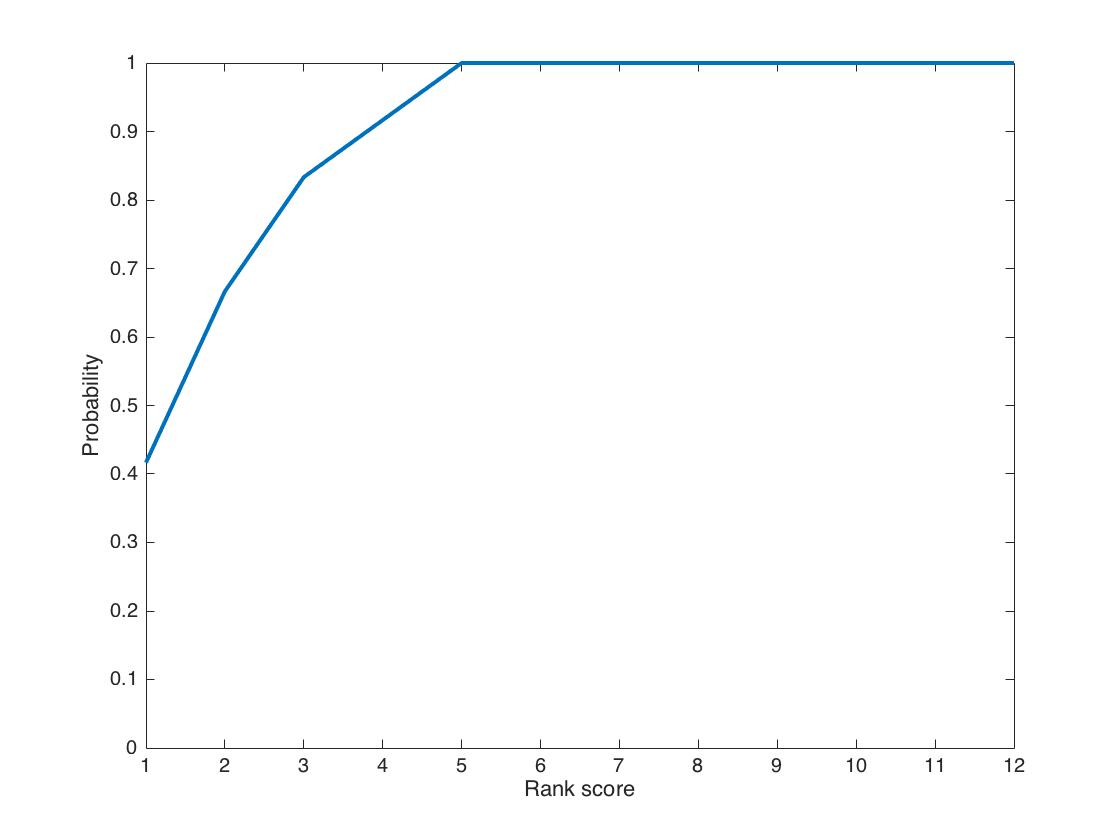
\includegraphics[width=1\linewidth]{/Users/JohnsonJohnson/Downloads/thesis_1/Figures/CMCexplanation.jpg}
\caption{A CMC plot of  gallery size is $M=10$ and probe size is $N=12$}
\label{CMCexplanationplot}
\vspace{-1em}
\end{figure} 






